\documentclass{standalone}
\usepackage{tikz}
\usetikzlibrary{patterns, positioning}

\begin{document}
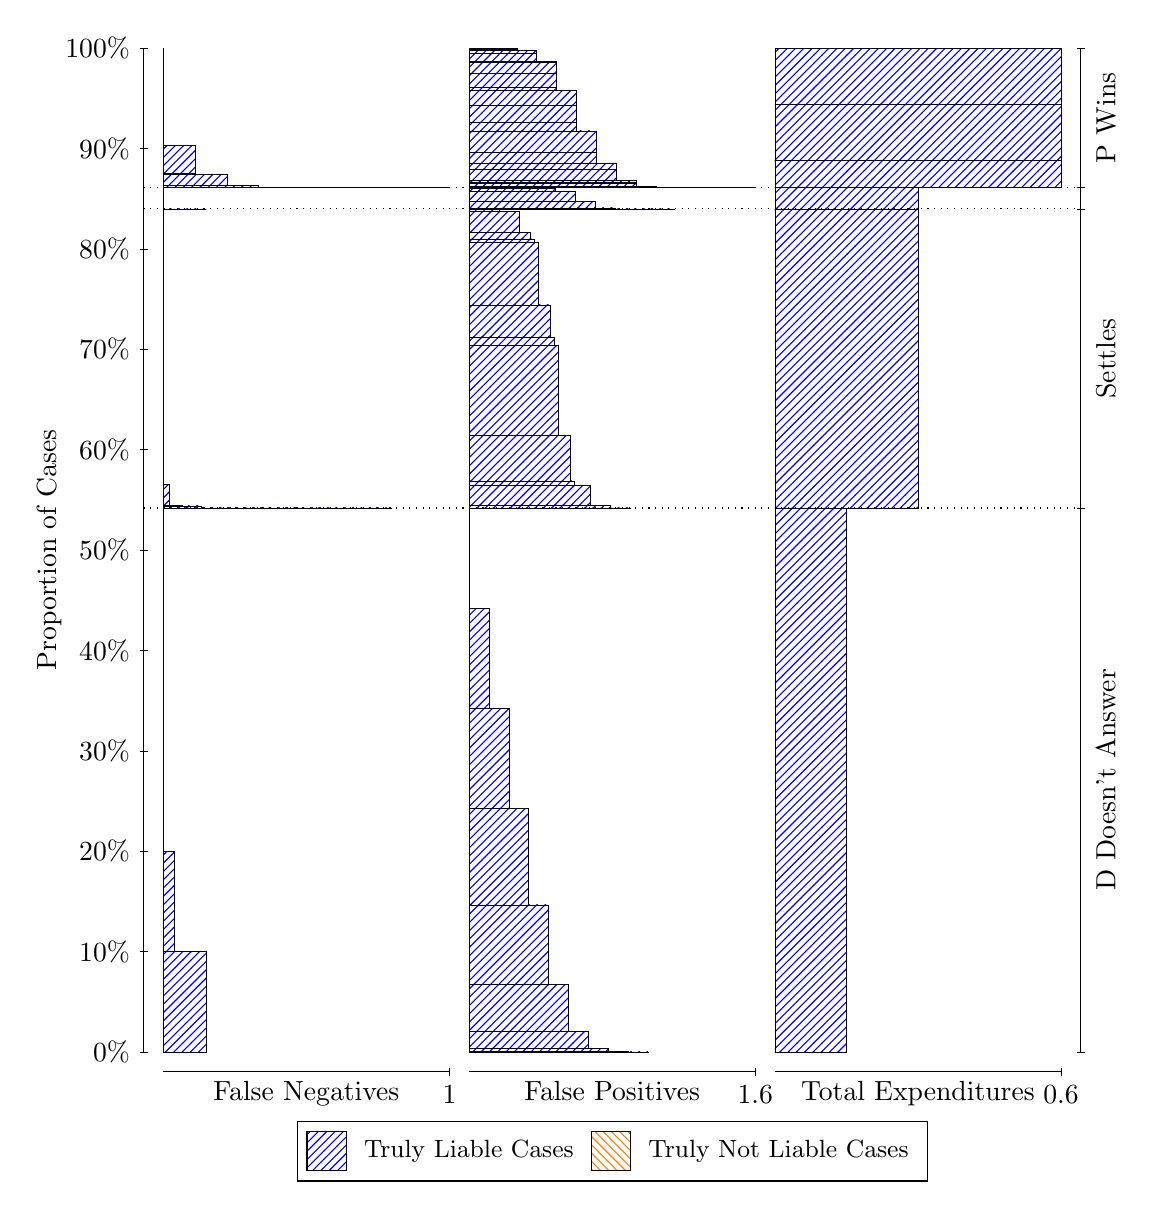
\begin{tikzpicture}
\draw[black, very thin] (1.5,1.75) -- (1.5,14.5);
\node[rotate=90, anchor=center] at (0.3, 8.125) {Proportion of Cases};
\draw[black, very thin] (1.45,1.75) -- (1.55,1.75);
\node[anchor=east] at (1.45, 1.75) {0\%};
\draw[black, very thin] (1.45,3.025) -- (1.55,3.025);
\node[anchor=east] at (1.45, 3.025) {10\%};
\draw[black, very thin] (1.45,4.3) -- (1.55,4.3);
\node[anchor=east] at (1.45, 4.3) {20\%};
\draw[black, very thin] (1.45,5.575) -- (1.55,5.575);
\node[anchor=east] at (1.45, 5.575) {30\%};
\draw[black, very thin] (1.45,6.85) -- (1.55,6.85);
\node[anchor=east] at (1.45, 6.85) {40\%};
\draw[black, very thin] (1.45,8.125) -- (1.55,8.125);
\node[anchor=east] at (1.45, 8.125) {50\%};
\draw[black, very thin] (1.45,9.4) -- (1.55,9.4);
\node[anchor=east] at (1.45, 9.4) {60\%};
\draw[black, very thin] (1.45,10.675) -- (1.55,10.675);
\node[anchor=east] at (1.45, 10.675) {70\%};
\draw[black, very thin] (1.45,11.95) -- (1.55,11.95);
\node[anchor=east] at (1.45, 11.95) {80\%};
\draw[black, very thin] (1.45,13.225) -- (1.55,13.225);
\node[anchor=east] at (1.45, 13.225) {90\%};
\draw[black, very thin] (1.45,14.5) -- (1.55,14.5);
\node[anchor=east] at (1.45, 14.5) {100\%};

\draw[black, very thin] (13.4,1.75) -- (13.4,14.5);
\draw[black, very thin] (13.35,1.75) -- (13.45,1.75);
\node[anchor=west] at (13.35, 1.75) {};
\draw[black, very thin] (13.35,8.659) -- (13.45,8.659);
\node[anchor=west] at (13.35, 8.659) {};
\draw[black, very thin] (13.35,12.457) -- (13.45,12.457);
\node[anchor=west] at (13.35, 12.457) {};
\draw[black, very thin] (13.35,12.726) -- (13.45,12.726);
\node[anchor=west] at (13.35, 12.726) {};
\draw[black, very thin] (13.35,14.5) -- (13.45,14.5);
\node[anchor=west] at (13.35, 14.5) {};

\draw[black, very thin, pattern color=blue, pattern=north east lines] (1.75,1.75) rectangle (2.295,3.025);
\draw[black, very thin, pattern color=blue, pattern=north east lines] (1.75,3.025) rectangle (1.8913,4.2998);
\draw[black, very thin, pattern color=orange, pattern=north west lines] (1.75,4.2998) rectangle (1.75,4.2998);
\draw[black, very thin, pattern color=blue, pattern=north east lines] (1.75,4.2998) rectangle (1.75,8.659);
\draw[black, very thin, pattern color=blue, pattern=north east lines] (1.75,8.659) rectangle (4.6567,8.659);
\draw[black, very thin, pattern color=blue, pattern=north east lines] (1.75,8.659) rectangle (4.253,8.659);
\draw[black, very thin, pattern color=blue, pattern=north east lines] (1.75,8.659) rectangle (3.93,8.659);
\draw[black, very thin, pattern color=blue, pattern=north east lines] (1.75,8.659) rectangle (3.8493,8.659);
\draw[black, very thin, pattern color=blue, pattern=north east lines] (1.75,8.659) rectangle (3.5263,8.659);
\draw[black, very thin, pattern color=blue, pattern=north east lines] (1.75,8.659) rectangle (3.4456,8.659);
\draw[black, very thin, pattern color=blue, pattern=north east lines] (1.75,8.659) rectangle (3.2033,8.659);
\draw[black, very thin, pattern color=blue, pattern=north east lines] (1.75,8.659) rectangle (3.1226,8.659);
\draw[black, very thin, pattern color=blue, pattern=north east lines] (1.75,8.659) rectangle (3.0419,8.659);
\draw[black, very thin, pattern color=blue, pattern=north east lines] (1.75,8.659) rectangle (2.7996,8.659);
\draw[black, very thin, pattern color=blue, pattern=north east lines] (1.75,8.659) rectangle (2.7189,8.659);
\draw[black, very thin, pattern color=blue, pattern=north east lines] (1.75,8.659) rectangle (2.6381,8.6595);
\draw[black, very thin, pattern color=blue, pattern=north east lines] (1.75,8.6595) rectangle (2.3959,8.6596);
\draw[black, very thin, pattern color=blue, pattern=north east lines] (1.75,8.6596) rectangle (2.3152,8.6596);
\draw[black, very thin, pattern color=blue, pattern=north east lines] (1.75,8.6596) rectangle (2.2344,8.6858);
\draw[black, very thin, pattern color=blue, pattern=north east lines] (1.75,8.6858) rectangle (1.9922,8.6894);
\draw[black, very thin, pattern color=blue, pattern=north east lines] (1.75,8.6894) rectangle (1.9115,8.6931);
\draw[black, very thin, pattern color=blue, pattern=north east lines] (1.75,8.6931) rectangle (1.8307,8.9606);
\draw[black, very thin, pattern color=orange, pattern=north west lines] (1.75,8.9606) rectangle (1.75,8.9606);
\draw[black, very thin, pattern color=blue, pattern=north east lines] (1.75,8.9606) rectangle (1.75,12.457);
\draw[black, very thin, pattern color=blue, pattern=north east lines] (1.75,12.457) rectangle (2.295,12.457);
\draw[black, very thin, pattern color=blue, pattern=north east lines] (1.75,12.457) rectangle (1.8913,12.457);
\draw[black, very thin, pattern color=orange, pattern=north west lines] (1.75,12.457) rectangle (1.75,12.457);
\draw[black, very thin, pattern color=blue, pattern=north east lines] (1.75,12.457) rectangle (1.75,12.726);
\draw[black, very thin, pattern color=blue, pattern=north east lines] (1.75,12.726) rectangle (5.3833,12.726);
\draw[black, very thin, pattern color=blue, pattern=north east lines] (1.75,12.726) rectangle (4.9796,12.726);
\draw[black, very thin, pattern color=blue, pattern=north east lines] (1.75,12.726) rectangle (4.5759,12.726);
\draw[black, very thin, pattern color=blue, pattern=north east lines] (1.75,12.726) rectangle (4.5759,12.726);
\draw[black, very thin, pattern color=blue, pattern=north east lines] (1.75,12.726) rectangle (4.1722,12.726);
\draw[black, very thin, pattern color=blue, pattern=north east lines] (1.75,12.726) rectangle (4.1722,12.726);
\draw[black, very thin, pattern color=blue, pattern=north east lines] (1.75,12.726) rectangle (3.7685,12.726);
\draw[black, very thin, pattern color=blue, pattern=north east lines] (1.75,12.726) rectangle (3.3648,12.726);
\draw[black, very thin, pattern color=blue, pattern=north east lines] (1.75,12.726) rectangle (3.3648,12.728);
\draw[black, very thin, pattern color=blue, pattern=north east lines] (1.75,12.728) rectangle (2.9611,12.73);
\draw[black, very thin, pattern color=blue, pattern=north east lines] (1.75,12.73) rectangle (2.9611,12.753);
\draw[black, very thin, pattern color=blue, pattern=north east lines] (1.75,12.753) rectangle (2.9611,12.753);
\draw[black, very thin, pattern color=blue, pattern=north east lines] (1.75,12.753) rectangle (2.5574,12.759);
\draw[black, very thin, pattern color=blue, pattern=north east lines] (1.75,12.759) rectangle (2.5574,12.896);
\draw[black, very thin, pattern color=blue, pattern=north east lines] (1.75,12.896) rectangle (2.1537,12.909);
\draw[black, very thin, pattern color=blue, pattern=north east lines] (1.75,12.909) rectangle (2.1537,13.266);
\draw[black, very thin, pattern color=blue, pattern=north east lines] (1.75,13.266) rectangle (2.1537,13.268);
\draw[black, very thin, pattern color=orange, pattern=north west lines] (1.75,13.268) rectangle (1.75,13.268);
\draw[black, very thin, pattern color=blue, pattern=north east lines] (1.75,13.268) rectangle (1.75,14.5);
\draw[black, very thin, pattern color=orange, pattern=north west lines] (5.6333,1.75) rectangle (7.9042,1.75);
\draw[black, very thin, pattern color=blue, pattern=north east lines] (5.6333,1.75) rectangle (7.9042,1.7502);
\draw[black, very thin, pattern color=blue, pattern=north east lines] (5.6333,1.7502) rectangle (7.6519,1.7539);
\draw[black, very thin, pattern color=blue, pattern=north east lines] (5.6333,1.7539) rectangle (7.3995,1.7944);
\draw[black, very thin, pattern color=blue, pattern=north east lines] (5.6333,1.7944) rectangle (7.1472,2.0086);
\draw[black, very thin, pattern color=blue, pattern=north east lines] (5.6333,2.0086) rectangle (6.8949,2.6062);
\draw[black, very thin, pattern color=blue, pattern=north east lines] (5.6333,2.6062) rectangle (6.6426,3.6168);
\draw[black, very thin, pattern color=blue, pattern=north east lines] (5.6333,3.6168) rectangle (6.3903,4.8389);
\draw[black, very thin, pattern color=blue, pattern=north east lines] (5.6333,4.8389) rectangle (6.138,6.1092);
\draw[black, very thin, pattern color=blue, pattern=north east lines] (5.6333,6.1092) rectangle (5.8856,7.384);
\draw[black, very thin, pattern color=blue, pattern=north east lines] (5.6333,7.384) rectangle (5.6333,8.659);
\draw[black, very thin, pattern color=orange, pattern=north west lines] (5.6333,8.659) rectangle (7.6771,8.659);
\draw[black, very thin, pattern color=blue, pattern=north east lines] (5.6333,8.659) rectangle (7.6771,8.6601);
\draw[black, very thin, pattern color=blue, pattern=north east lines] (5.6333,8.6601) rectangle (7.4248,8.689);
\draw[black, very thin, pattern color=orange, pattern=north west lines] (5.6333,8.689) rectangle (7.2229,8.689);
\draw[black, very thin, pattern color=blue, pattern=north east lines] (5.6333,8.689) rectangle (7.2229,8.6992);
\draw[black, very thin, pattern color=blue, pattern=north east lines] (5.6333,8.6992) rectangle (7.1725,8.9442);
\draw[black, very thin, pattern color=blue, pattern=north east lines] (5.6333,8.9442) rectangle (6.9706,9.0028);
\draw[black, very thin, pattern color=blue, pattern=north east lines] (5.6333,9.0028) rectangle (6.9201,9.5817);
\draw[black, very thin, pattern color=orange, pattern=north west lines] (5.6333,9.5817) rectangle (6.7687,9.5817);
\draw[black, very thin, pattern color=blue, pattern=north east lines] (5.6333,9.5817) rectangle (6.7687,10.723);
\draw[black, very thin, pattern color=blue, pattern=north east lines] (5.6333,10.723) rectangle (6.7183,10.831);
\draw[black, very thin, pattern color=blue, pattern=north east lines] (5.6333,10.831) rectangle (6.6678,11.238);
\draw[black, very thin, pattern color=blue, pattern=north east lines] (5.6333,11.238) rectangle (6.5164,12.031);
\draw[black, very thin, pattern color=blue, pattern=north east lines] (5.6333,12.031) rectangle (6.466,12.075);
\draw[black, very thin, pattern color=blue, pattern=north east lines] (5.6333,12.075) rectangle (6.4155,12.155);
\draw[black, very thin, pattern color=blue, pattern=north east lines] (5.6333,12.155) rectangle (6.2641,12.422);
\draw[black, very thin, pattern color=blue, pattern=north east lines] (5.6333,12.422) rectangle (6.2137,12.426);
\draw[black, very thin, pattern color=blue, pattern=north east lines] (5.6333,12.426) rectangle (6.1632,12.43);
\draw[black, very thin, pattern color=blue, pattern=north east lines] (5.6333,12.43) rectangle (6.0118,12.456);
\draw[black, very thin, pattern color=blue, pattern=north east lines] (5.6333,12.456) rectangle (5.9613,12.456);
\draw[black, very thin, pattern color=blue, pattern=north east lines] (5.6333,12.456) rectangle (5.9109,12.456);
\draw[black, very thin, pattern color=blue, pattern=north east lines] (5.6333,12.456) rectangle (5.7595,12.457);
\draw[black, very thin, pattern color=blue, pattern=north east lines] (5.6333,12.457) rectangle (5.709,12.457);
\draw[black, very thin, pattern color=blue, pattern=north east lines] (5.6333,12.457) rectangle (5.6586,12.457);
\draw[black, very thin, pattern color=blue, pattern=north east lines] (5.6333,12.457) rectangle (5.6333,12.457);
\draw[black, very thin, pattern color=orange, pattern=north west lines] (5.6333,12.457) rectangle (8.2448,12.457);
\draw[black, very thin, pattern color=blue, pattern=north east lines] (5.6333,12.457) rectangle (8.2448,12.457);
\draw[black, very thin, pattern color=blue, pattern=north east lines] (5.6333,12.457) rectangle (7.9925,12.457);
\draw[black, very thin, pattern color=blue, pattern=north east lines] (5.6333,12.457) rectangle (7.7402,12.457);
\draw[black, very thin, pattern color=blue, pattern=north east lines] (5.6333,12.457) rectangle (7.4878,12.469);
\draw[black, very thin, pattern color=blue, pattern=north east lines] (5.6333,12.469) rectangle (7.2355,12.556);
\draw[black, very thin, pattern color=blue, pattern=north east lines] (5.6333,12.556) rectangle (6.9832,12.679);
\draw[black, very thin, pattern color=blue, pattern=north east lines] (5.6333,12.679) rectangle (6.7309,12.721);
\draw[black, very thin, pattern color=blue, pattern=north east lines] (5.6333,12.721) rectangle (6.4786,12.725);
\draw[black, very thin, pattern color=blue, pattern=north east lines] (5.6333,12.725) rectangle (6.2263,12.726);
\draw[black, very thin, pattern color=blue, pattern=north east lines] (5.6333,12.726) rectangle (5.974,12.726);
\draw[black, very thin, pattern color=orange, pattern=north west lines] (5.6333,12.726) rectangle (9.2667,12.726);
\draw[black, very thin, pattern color=blue, pattern=north east lines] (5.6333,12.726) rectangle (9.2667,12.726);
\draw[black, very thin, pattern color=orange, pattern=north west lines] (5.6333,12.726) rectangle (9.0144,12.726);
\draw[black, very thin, pattern color=blue, pattern=north east lines] (5.6333,12.726) rectangle (9.0144,12.726);
\draw[black, very thin, pattern color=orange, pattern=north west lines] (5.6333,12.726) rectangle (8.762,12.726);
\draw[black, very thin, pattern color=blue, pattern=north east lines] (5.6333,12.726) rectangle (8.762,12.726);
\draw[black, very thin, pattern color=blue, pattern=north east lines] (5.6333,12.726) rectangle (8.5097,12.726);
\draw[black, very thin, pattern color=orange, pattern=north west lines] (5.6333,12.726) rectangle (8.5097,12.726);
\draw[black, very thin, pattern color=blue, pattern=north east lines] (5.6333,12.726) rectangle (8.5097,12.726);
\draw[black, very thin, pattern color=blue, pattern=north east lines] (5.6333,12.726) rectangle (8.2574,12.727);
\draw[black, very thin, pattern color=orange, pattern=north west lines] (5.6333,12.727) rectangle (8.2574,12.727);
\draw[black, very thin, pattern color=blue, pattern=north east lines] (5.6333,12.727) rectangle (8.2574,12.728);
\draw[black, very thin, pattern color=blue, pattern=north east lines] (5.6333,12.728) rectangle (8.0051,12.734);
\draw[black, very thin, pattern color=orange, pattern=north west lines] (5.6333,12.734) rectangle (8.0051,12.734);
\draw[black, very thin, pattern color=blue, pattern=north east lines] (5.6333,12.734) rectangle (8.0051,12.745);
\draw[black, very thin, pattern color=blue, pattern=north east lines] (5.6333,12.745) rectangle (7.7528,12.745);
\draw[black, very thin, pattern color=orange, pattern=north west lines] (5.6333,12.745) rectangle (7.7528,12.745);
\draw[black, very thin, pattern color=blue, pattern=north east lines] (5.6333,12.745) rectangle (7.7528,12.777);
\draw[black, very thin, pattern color=blue, pattern=north east lines] (5.6333,12.777) rectangle (7.7528,12.801);
\draw[black, very thin, pattern color=blue, pattern=north east lines] (5.6333,12.801) rectangle (7.7528,12.819);
\draw[black, very thin, pattern color=blue, pattern=north east lines] (5.6333,12.819) rectangle (7.5005,12.82);
\draw[black, very thin, pattern color=orange, pattern=north west lines] (5.6333,12.82) rectangle (7.5005,12.82);
\draw[black, very thin, pattern color=blue, pattern=north east lines] (5.6333,12.82) rectangle (7.5005,12.964);
\draw[black, very thin, pattern color=blue, pattern=north east lines] (5.6333,12.964) rectangle (7.5005,13.036);
\draw[black, very thin, pattern color=blue, pattern=north east lines] (5.6333,13.036) rectangle (7.2481,13.036);
\draw[black, very thin, pattern color=blue, pattern=north east lines] (5.6333,13.036) rectangle (7.2481,13.173);
\draw[black, very thin, pattern color=orange, pattern=north west lines] (5.6333,13.173) rectangle (7.2481,13.173);
\draw[black, very thin, pattern color=blue, pattern=north east lines] (5.6333,13.173) rectangle (7.2481,13.448);
\draw[black, very thin, pattern color=blue, pattern=north east lines] (5.6333,13.448) rectangle (6.9958,13.553);
\draw[black, very thin, pattern color=orange, pattern=north west lines] (5.6333,13.553) rectangle (6.9958,13.553);
\draw[black, very thin, pattern color=blue, pattern=north east lines] (5.6333,13.553) rectangle (6.9958,13.774);
\draw[black, very thin, pattern color=blue, pattern=north east lines] (5.6333,13.774) rectangle (6.9958,13.958);
\draw[black, very thin, pattern color=blue, pattern=north east lines] (5.6333,13.958) rectangle (6.7435,13.996);
\draw[black, very thin, pattern color=blue, pattern=north east lines] (5.6333,13.996) rectangle (6.7435,14.179);
\draw[black, very thin, pattern color=blue, pattern=north east lines] (5.6333,14.179) rectangle (6.7435,14.316);
\draw[black, very thin, pattern color=blue, pattern=north east lines] (5.6333,14.316) rectangle (6.7435,14.329);
\draw[black, very thin, pattern color=blue, pattern=north east lines] (5.6333,14.329) rectangle (6.4912,14.427);
\draw[black, very thin, pattern color=blue, pattern=north east lines] (5.6333,14.427) rectangle (6.4912,14.472);
\draw[black, very thin, pattern color=blue, pattern=north east lines] (5.6333,14.472) rectangle (6.4912,14.473);
\draw[black, very thin, pattern color=blue, pattern=north east lines] (5.6333,14.473) rectangle (6.2389,14.473);
\draw[black, very thin, pattern color=blue, pattern=north east lines] (5.6333,14.473) rectangle (6.2389,14.489);
\draw[black, very thin, pattern color=blue, pattern=north east lines] (5.6333,14.489) rectangle (6.2389,14.498);
\draw[black, very thin, pattern color=blue, pattern=north east lines] (5.6333,14.498) rectangle (6.2389,14.498);
\draw[black, very thin, pattern color=blue, pattern=north east lines] (5.6333,14.498) rectangle (5.9866,14.499);
\draw[black, very thin, pattern color=blue, pattern=north east lines] (5.6333,14.499) rectangle (5.9866,14.5);
\draw[black, very thin, pattern color=blue, pattern=north east lines] (5.6333,14.5) rectangle (5.7343,14.5);
\draw[black, very thin, pattern color=blue, pattern=north east lines] (5.6333,14.5) rectangle (5.7343,14.5);
\draw[black, very thin, pattern color=blue, pattern=north east lines] (5.6333,14.5) rectangle (5.7343,14.5);
\draw[black, very thin, pattern color=blue, pattern=north east lines] (5.6333,14.5) rectangle (5.6333,14.5);
\draw[black, very thin, pattern color=orange, pattern=north west lines] (9.5167,1.75) rectangle (10.425,1.75);
\draw[black, very thin, pattern color=blue, pattern=north east lines] (9.5167,1.75) rectangle (10.425,8.659);
\draw[black, very thin, pattern color=orange, pattern=north west lines] (9.5167,8.659) rectangle (11.333,8.659);
\draw[black, very thin, pattern color=blue, pattern=north east lines] (9.5167,8.659) rectangle (11.333,12.457);
\draw[black, very thin, pattern color=orange, pattern=north west lines] (9.5167,12.457) rectangle (11.333,12.457);
\draw[black, very thin, pattern color=blue, pattern=north east lines] (9.5167,12.457) rectangle (11.333,12.726);
\draw[black, very thin, pattern color=orange, pattern=north west lines] (9.5167,12.726) rectangle (13.15,12.726);
\draw[black, very thin, pattern color=blue, pattern=north east lines] (9.5167,12.726) rectangle (13.15,13.077);
\draw[black, very thin, pattern color=orange, pattern=north west lines] (9.5167,13.077) rectangle (13.15,13.077);
\draw[black, very thin, pattern color=blue, pattern=north east lines] (9.5167,13.077) rectangle (13.15,13.785);
\draw[black, very thin, pattern color=orange, pattern=north west lines] (9.5167,13.785) rectangle (13.15,13.785);
\draw[black, very thin, pattern color=blue, pattern=north east lines] (9.5167,13.785) rectangle (13.15,14.5);
\draw[black, dotted] (1.5,8.659) -- (13.4,8.659);
\draw[black, dotted] (1.5,12.457) -- (13.4,12.457);
\draw[black, dotted] (1.5,12.726) -- (13.4,12.726);
\draw[black, very thin] (1.75,1.5) -- (5.3833,1.5);
\node[anchor=north] at (3.5667, 1.5) {False Negatives};
\draw[black, very thin] (5.3833,1.45) -- (5.3833,1.55);
\node[anchor=north] at (5.3833, 1.45) {1};

\draw[black, very thin] (5.6333,1.5) -- (9.2667,1.5);
\node[anchor=north] at (7.45, 1.5) {False Positives};
\draw[black, very thin] (9.2667,1.45) -- (9.2667,1.55);
\node[anchor=north] at (9.2667, 1.45) {1.6};

\draw[black, very thin] (9.5167,1.5) -- (13.15,1.5);
\node[anchor=north] at (11.333, 1.5) {Total Expenditures};
\draw[black, very thin] (13.15,1.45) -- (13.15,1.55);
\node[anchor=north] at (13.15, 1.45) {0.6};

\node[black, centered, rotate=90] at (13.72, 5.2045) {D Doesn't Answer};
\node[black, centered, rotate=90] at (13.72, 10.558) {Settles};

\node[black, centered, rotate=90] at (13.72, 13.613) {P Wins};

\draw (7.449999999999999,1.5) node[draw=none] (baseCoordinate) {};
\begin{scope}[align=center]
        \matrix[scale=0.5, draw=black, below=0.5cm of baseCoordinate, nodes={draw}, column sep=0.1cm]{
            \node[rectangle, draw, minimum width=0.5cm, minimum height=0.5cm, pattern=north east lines, pattern color=blue] {}; &
            \node[draw=none, font=\small] (B) {Truly Liable Cases}; &
            \node[rectangle, draw, minimum width=0.5cm, minimum height=0.5cm, pattern=north west lines, pattern color=orange] {}; &
            \node[draw=none, font=\small] (B) {Truly Not Liable Cases}; \\
            };
\end{scope}

\end{tikzpicture}
\end{document}